\section{Implementation and Results} \label{imple}


\begin{table}[b]
\centering
\caption{List of Benchmark programs used as real time tasks}
\scalebox{0.9}{
\begin{tabular}{|c|c|c|c|} \hline
\bf{Benchmark} & \bf{Total}  & \bf{Memory} & \bf{Memory}\\ 
\bf{programs} & \bf{instructions} & \bf{Reads} & \bf{Writes} \\ \hline
bs & 179 & 32 & 32 \\ \hline
cnt & 295 & 52 & 43 \\ \hline
duff & 257 & 47 & 64 \\ \hline
fac & 164 & 24 & 24 \\ \hline
fibcall & 163 & 27 & 28 \\ \hline
insertsort & 189 & 36 & 30\\ \hline
lcdnum & 198 & 26 & 23 \\ \hline
ns & 245 & 31 & 40 \\ \hline
prime & 226 & 28 & 41 \\ \hline
res & 179 & 91 & 88 \\ \hline
\end{tabular}
}
\label{bench}
\end{table}




\begin{table}
\begin{flushleft}
\caption{Results on some of the Datasets}
\scalebox{0.9}{
 \begin{tabular}{|c|c|c|c|c|c|}\hline
 \bf{Dataset} & \bf{Number} & \bf{Number} & \bf{Rowsize} & \bf{Number} & \bf{Number} \\
 \bf{Number}  &  \bf{of}  & \bf{of}  & & \bf{of Task} & \bf{of Task} \\ 
         &  \bf{cycles} & \bf{Banks} &  & \bf{Miss}&\bf{Miss}  \\
         &        &       &    & \bf{(open-page}& \bf{(our} \\         
         &         &       &  & \bf{policy)}         &  \bf{method)}\\
 \hline Dataset I & 10,000 & 10 banks & 64B & 1 & 1 \\
 (fibcall.c,& 20,000 &          &     & 3 & 2 \\
  lcdnum.c,&30,000 &          &      & 4 & 3 \\
  fac.c)   &40,000 &          &      & 6 & 4 \\
           & 50,000 &        &       & 8 & 5 \\
           & 60,000 &        &      & 9 & 6 \\
           & 70,000 &        &      & 11 & 7 \\ \hline
           & 10,000 & 10 banks & 32B & 2 & 1 \\ 
           & 20,000 &        &       & 4 & 2 \\
           & 30,000 &        &       & 5 & 3 \\
           & 40,000 &        &       & 8 & 5 \\
           & 50,000 &        &       & 11 & 6 \\
           & 60,000 &        &       & 12 & 7 \\
           & 70,000 &        &       & 14 & 9 \\ \hline
 Dataset II & 10,000 & 19 banks & 64B & 3 & 0 \\
 (bs.c,     & 20,000 &         &      & 6 & 1 \\
  count.c   & 30,000 &         &      & 9 & 1 \\
  duff.c)   & 40,000 &         &      & 14 & 4 \\ \hline
            & 10,000 & 19 banks & 32B & 3 & 2 \\
            & 20,000 &          &     & 5 & 3 \\
            & 30,000 &          &     & 8 & 6 \\
            & 40,000 &          &     & 13 & 11 \\ \hline
 Dataset III & 10,000 & 15 banks & 64B & 2 & 1 \\
 (prime.c,   & 20,000 &          &     & 4 & 1 \\
  ns.c,      & 30,000 &          &     & 5 & 2 \\
  insertsort.c)& 40,000 &          &     & 8 & 3 \\ \hline
             &10,000 & 15 banks & 32B & 3 & 2 \\  
             & 20,000&          &     & 5 & 3 \\
             & 30,000&          &     & 6 & 4 \\
             & 40,000&          &     & 9 & 6 \\ \hline
 Dataset IV  & 10,000& 12 banks & 64B & 2 & 1 \\
 (lcdnum.c,  & 20,000 &         &     & 5 & 2 \\
  insertsort.c,& 30,000 &         &     & 7 & 4 \\
  fibcall.c) & 40,000 &         &     & 12 & 4 \\ \hline
             &10,000 & 12 banks & 32B & 3 & 2 \\
             & 20,000 &         &     & 6 & 4 \\
             & 30,000 &         &     & 9 & 6 \\
             & 40,000 &         &     & 14 & 11\\ \hline  
 \end{tabular}
 }
\end{flushleft}
\label{Data_results}
\end{table}


\noindent
Our end to end implementation consists of two main parts. The first part consists of trace generation from benchmark programs 
of the Malardalen WCET benchmark~\cite{gustafsson2010malardalen}. We executed our benchmark programs on an X-86 architectural 
platform to generate X-86 instructions. Table~\ref{bench} gives a description of the benchmark programs in detail. 
In our implementation, the arrival time (A) of each task is randomly generated. The execution time of a task(E) is actually the 
sum of execution time of all the instructions in the worst case. The period of each task (P) is randomly generated with the 
condition that it should 
be greater than the worst case execution time. We have considered the deadline of a task instance (D) to be equal to 
the period after which the next task instance arrives. Thus at a particular time instant only one task 
instance of a task actually executes in the system. 
%A diagrammatic view of our trace generation is shown in Fig \ref{fig5}. 
The final part deals with the end to end simulation. 
We have considered a uni-processor system, where tasks are scheduled according to EDF at the processor. Whenever a memory 
request arrives, a context switch occurs at the CPU and the memory request waits in the memory buffer. The memory controller 
then selects a request from the memory buffer based on our proposed algorithm and executes a task in memory. Our results were
generated by varying the number of banks and the size of row in each bank. In all the cases, we have assumed that we have a set 
of two extra banks which do not participate in address mapping. We have 
implemented our own end-to-end simulator and have compared our results with existing state-of-the-art DRAM controllers. 
Table \ref{Data_results} shows a comparative analysis of existing DRAM controllers following open-page policy vs our proposed DRAM 
controller. We have generated some dataset from the benchmark programs of the Malardalen WCET benchmark. We have run each dataset
upto certain number of cycles by varying the number of memory banks. We have also varied the size of each row in a memory bank.
In Table \ref{Data_results}, column I shows the programs in each dataset, column II shows the number of cycles upto which we ran our 
experiments, column III shows the number of banks in the memory module we worked on, column IV shows the size of row in each 
bank, column V shows the number of misses in DRAM with open-page policy and column VI shows the number of misses we achieved by using 
our scheduling algorithm at the DRAM controller.



%\begin{figure}
% \centering
%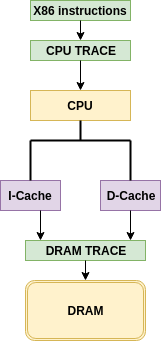
\includegraphics[width=3.5cm,height=4.2cm]{TRACE.png}
% \caption{Overview of Trace Generation}
% \label{fig5}
%\end{figure}





